
Der USB Gadget Modus der Raspberry Pi Zero ist bereits auf dem Raspjamming Image vorinstalliert. Die Vergabe der IP-Adresse erfolgt �ber einen DHCP-Server, sodass im Idealfall keinerlei Einstellungen am Host System vorgenommen werden m�ssen.\\
Nur das Weiterleiten des Internets auf die Netzwerkverbindung des Raspberry Pi Zero ist manuell   einzurichten.\\
Auch wenn der Raspberry Pi �ber WLAN mit dem lokalen Netz verbunden ist, ist der folgende Einrichtungsvorgang identisch. Nur das weiterleiten des Internets ist dann nicht n�tig.  


%\subsection{Host (DHCP-Client)}
%\clearpage
%\subsubsection{Kubuntu 16.04}

Am Host-PC muss bei den IPv4-Einstellungen die Methode "`Automatisch"' eingestellt sein. Wenn es sich um eine neue Verbindung handelt, ist dies bereits voreingestellt, eine Parametrierung kann dann entfallen. Ansonsten muss zur Konfiguration unter Linux (Kubuntu 16.04) zuerst der Dialog "`Netzwerkverbindungen"' ge�ffnet werden.\\ 
Dazu klickt man mit der rechten Maustaste auf das Netzwerksymbol in Infobereich rechts unten. Dann kann die Option "`Netzwerkverbindungen einrichten..."' ausgew�hlt werden.

\begin{figure}[ht]
  \centering
  
\includegraphics[scale=1.00]{images/OTG_NetzwerkverbindungenIcon.png}	
  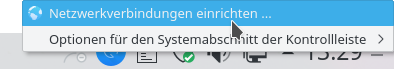
\includegraphics[scale=0.42]{images/OTG_NetzwerkverbindungenOpen.png}	
  %	\caption{}
  \label{OTG_LINUX_NetzwerkverbindungenApp}
\end{figure}


Nun k�nnte die neue "`Kabelnetzwerkverbindung"' umbenannt werden, z.~B. in Raspberry Pi Zero. Erkennen kann man das Netzwerk an der Mac-Adresse, die man bei "`g\_ether.host\_addr"' angegeben hat (z.~B. 00:01:02:03:04:05).  


\begin{figure}[ht]
  \centering
  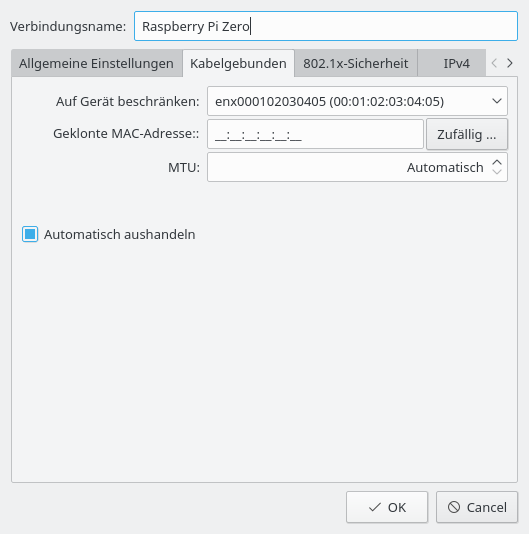
\includegraphics[scale=0.42]{images/OTG_Pi_Verbindungsname.png}
	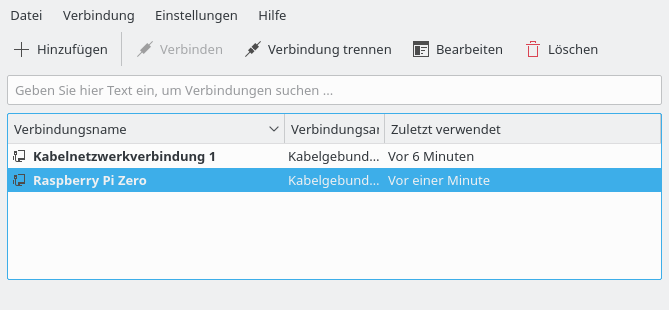
\includegraphics[scale=0.42]{images/OTG_Netzwerkverbindungen.png}
%	\caption{}
  \label{OTG_LINUX_Netzwerkverbindungen}
\end{figure}


Nun kann bei den IPv4-Einstellungen die Methode "`Automatisch"' eingestellt werden.

%\begin{figure}[ht]
%  \centering
%  \includegraphics[scale=0.42]{images/OTG_NetzwerkverbindungenAutomatisch.png}
%	\caption{}
%  \label{OTG_LINUX_Netzwerkverbindungen}
%\end{figure}

%\clearpage
\subsection{Linux (Mint XFCE)}

Am Host-PC muss bei den IPv4-Einstellungen die Methode "`Automatisch"' eingestellt sein. Wenn es sich um eine neue Verbindung handelt, ist dies bereits voreingestellt, eine Parametrierung kann dann entfallen. Ansonsten muss zur Konfiguration unter Linux (Mint XFCE) zuerst der Dialog "`Netzwerkverbindungen"' ge�ffnet werden.\\ 
Dazu klickt man mit der rechten Maustaste auf das Netzwerksymbol in Infobereich rechts unten. Dann kann die Option "`Netzwerkverbindungen bearbeiten..."' ausgew�hlt werden.

\begin{figure}[ht]
  \centering
  
\includegraphics[scale=1.00]{images/OTG_NetzwerkverbindungenIconMintXFCE.png}	
  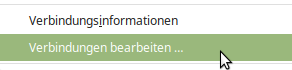
\includegraphics[scale=0.42]{images/OTG_NetzwerkverbindungenOpenMintXFCE.png}	
  %	\caption{}
  \label{OTG_LINUX_NetzwerkverbindungenApp}
\end{figure}


Nun k�nnte die neue "`Kabelnetzwerkverbindung 2"' umbenannt werden, z.~B. in Raspberry Pi Zero. Erkennen kann man das Netzwerk an der Mac-Adresse, die man bei "`g\_ether.host\_addr"' angegeben hat (z.~B. 00:01:02:03:04:05).  


\begin{figure}[ht]
  \centering
	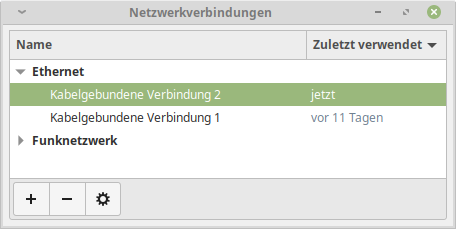
\includegraphics[scale=0.38]{images/OTG_NetzwerkverbindungenMintXFCE.png}
  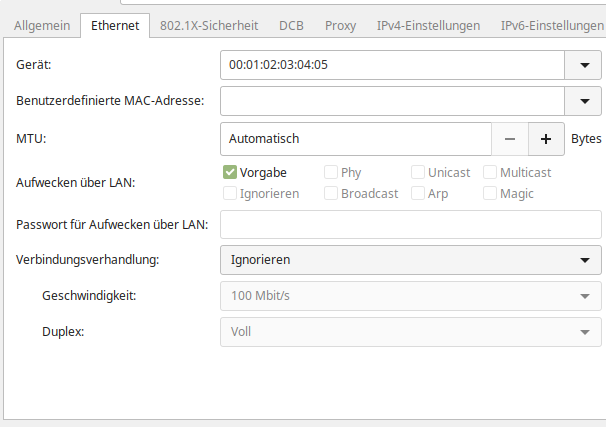
\includegraphics[scale=0.38]{images/OTG_Pi_VerbindungsnameMintXFCE.png}
%	\caption{}
  \label{OTG_LINUX_Netzwerkverbindungen}
\end{figure}


Nun kann bei den IPv4-Einstellungen die Methode "`Automatisch"' eingestellt werden.

\begin{figure}[ht]
  \centering
  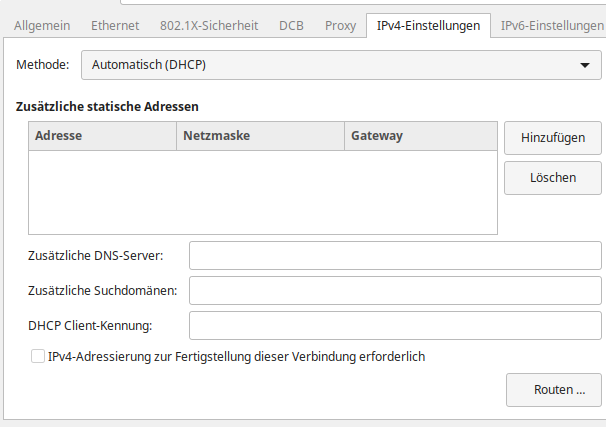
\includegraphics[scale=0.38]{images/OTG_NetzwerkverbindungenAutomatischMintXFCE.png}
%	\caption{}
  \label{OTG_LINUX_Netzwerkverbindungen_Auto}
\end{figure}


%\subsection{Internet Zugriff} 
~\\
Nach der Einrichtung des Netzwerk kann der Raspberry Pi Zero mit dem Namen "`raspberrypi.local"' erreicht werden. Um den Raspbery Pi Zero mit dem Internet verbinden zu k�nnen m�ssen einige Einstellungen am Host %und Client
 gemacht werden. Man muss den Name des Netzwerkger�ts am Host-PC kennen, das mit dem Internet verbunden ist. Dies ermittelt man �ber die Netzwerkeinstellungen oder �ber die Konsole mit nmcli. Im Beispielfall ist der Name "`enp0s25"' das richtige Ger�t.

\begin{console} 
	nmcli d
\end{console} 

\begin{screensmall} 
	GER�T            TYP       STATUS           VERBINDUNG        
	enx000102030405  ethernet  verbunden        Raspberry Pi Zero 
	enp0s25          ethernet  verbunden        Netzwerkverbindung 1                
	lo               loopback  nicht verwaltet  --  
\end{screensmall}

Damit der Internetzugang f�r den Raspberry Pi Zero freigegeben wird, m�ssen am Host-PC folgende Befehle in einem Terminal eingeben werden. "`enp0s25"' muss durch den Namen des Netzwerkger�ts ersetzt werden, das mit dem Internet verbunden ist.

\begin{console} 
	sudo sysctl -w net.ipv4.ip_forward=1
	sudo iptables -t nat -A POSTROUTING -o enp0s25 -j MASQUERADE
\end{console}



Alternativ k�nnen die Einstellungen auch automatisch �ber eine Shell-Script durchgef�hrt werden (siehe Kapitel \ref{sec:shellscript} \titleref{sec:shellscript}).

\subsection{Windows 10}

Nach dem Boot wird der Raspberry Pi Zero als "`Serielles USB-Ger�t"' erkannt und keine korrekten Treiber installiert. Dies muss manuell erfolgen. Dazu l�dt man sich zuerst den zertifizierten Treiber "`Acer Incorporated. - Other hardware - USB Ethernet-RNDIS Gadget"' von der Microsoft Homepage herunter \url{http://download.windowsupdate.com/msdownload/update/driver/drvs/2012/12/20342322_4b9970e3174b23b5cb2371af0837f939a71271ea.cab} bzw. \url{https://tinyurl.com/y6onwaax}. Die ben�tigten Dateien sind in der komprimierten CAB-Datei enthalten. Durch einen Doppelklick auf der Datei kann der Inhalt dargestellt werden. Mit der rechten Maustaste und dem Kontexmen� k�nnen die Dateien z.~B. nach \path{c:\Drivers\RNDIS\} extrahiert werden. 

\begin{figure}[ht]
  \centering
  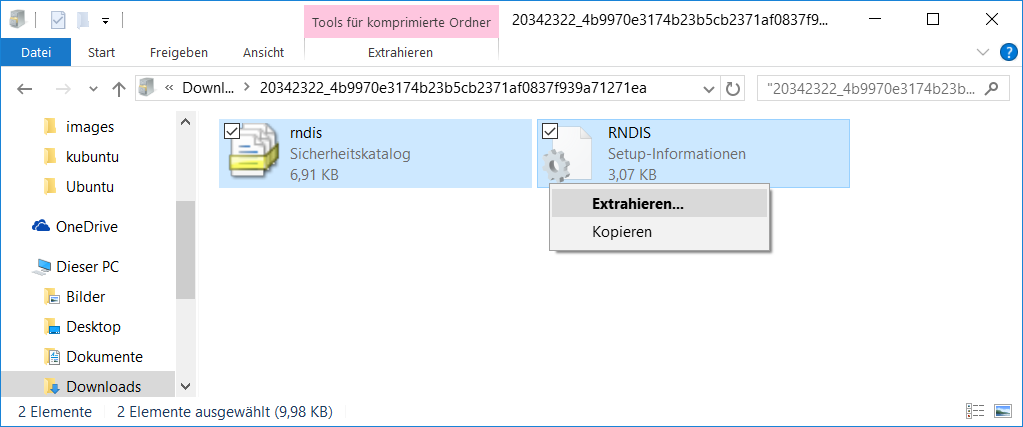
\includegraphics[scale=0.42]{images/OTG_Win10_Install_0.png}
%  \caption{}
  \label{OTG_Win10_Drivers}
\end{figure}

Nun muss der Gr�temanager ge�ffnet werden. Dann �ffnet man das Kontextmen� in dem man die rechte Maustaste am 
"`Serielles USB-Ger�t"' Eintrag dr�ckt. Nun w�hlt man den Men�punkt "`Treiber Software aktualisieren..."' aus. Im folgenden Dialog w�hlt man "`Auf dem Computer nach Treibersoftware suchen"' und dann gibt man das Verzeichnis an, in dem die Treiberdaten extrahiert wurden, z.~B. \path{c:\Drivers\RNDIS\}. Zum Schluss sollte der Treiber automatisch erfolgreich installiert werden.\\ 

\begin{figure}[ht]
  \centering
  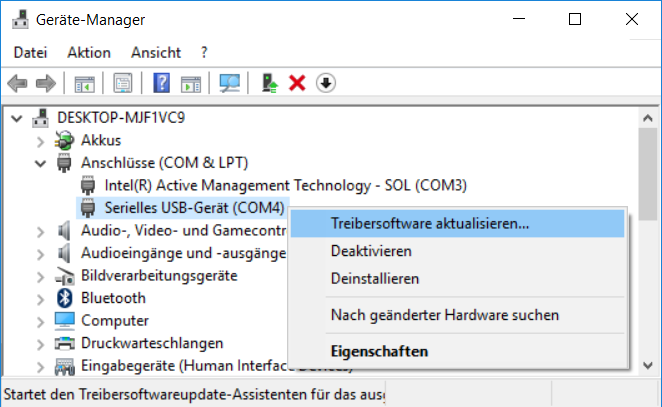
\includegraphics[scale=0.5]{images/OTG_Win10_Install_1.png}
  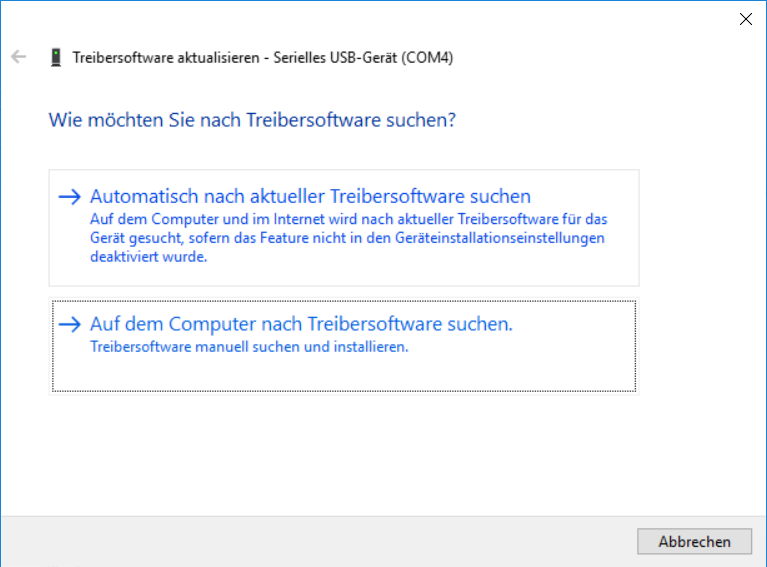
\includegraphics[scale=0.4]{images/OTG_Win10_Install_2.png}
%  \caption{}
  \label{OTG_Win10_Install_1}
\end{figure}


\begin{figure}[ht]
  \centering
  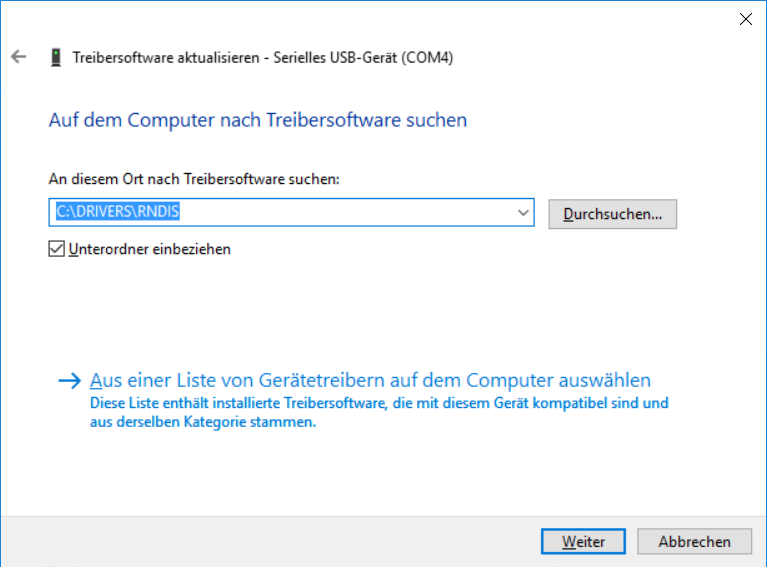
\includegraphics[scale=0.4]{images/OTG_Win10_Install_3.png}
  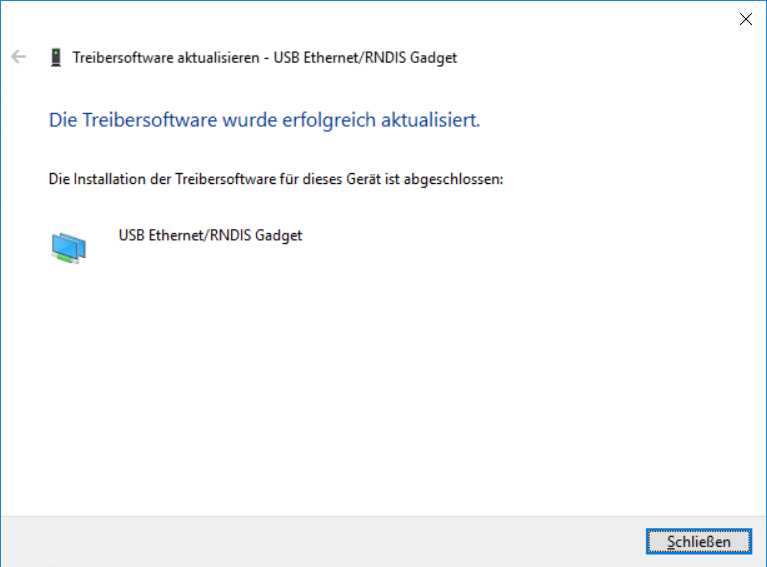
\includegraphics[scale=0.4]{images/OTG_Win10_Install_4.png}
%  \caption{}
  \label{OTG_Win10_Install_3}
\end{figure}  


Damit am Ger�t Internet funktionieren kann, muss das Internet f�r das neue Netzwerk freigegeben werden. Dazu �ffnet man das Einstellungs-Fenster f�r die Netzwerkverbindungen. 

\begin{figure}[ht]
  \centering
  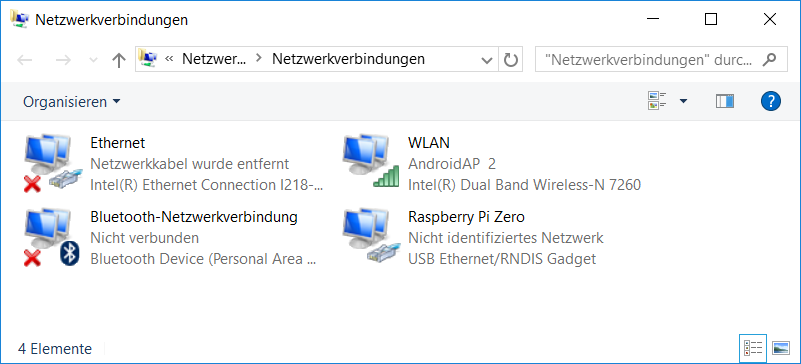
\includegraphics[scale=0.40]{images/OTG_Win10_Netzwerkverbindungen.png}
  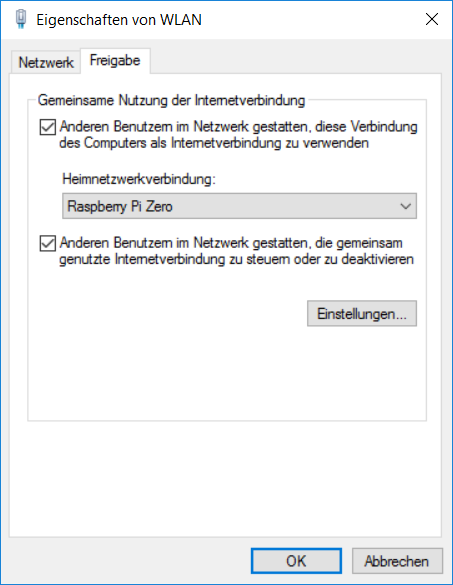
\includegraphics[scale=0.40]{images/OTG_Win10_Inet.png}
%	\caption{}
  \label{OTG_Win10_Netzwerkverbindungen}
\end{figure}

Zuerst kann man dem Netzwerkger�t "`USB Ethernet/RNDIS Gadget"' einen neuen Namen geben, z.~B. Raspberry Pi Zero. Nun muss das Netzwerk gesucht werden, das mit dem Internet verbunden ist, z.~B. WLAN. Bei den Eigenschaften zu dem Netzwerk kann der Reiter "`Freigabe"' ausgew�hlt werden. Danach kann man die Einstellung "`Anderen Benutzern im Netzwerk gestatten, diese Verbindung des Computers als Internetverbindung zu verwenden"' aktivieren und bei Heimnetzwerkverbindung kann das Netzwerk "`Raspberry Pi Zero"' ausgew�hlt werden.\\

Nun kann die Verbindung zur Raspberry Pi mit dem Programm Putty und der Adresse "`raspberrypi.local"', �ber das SSH-Protokoll hergestellt werden (siehe Kapitel \ref{sec:connection_putty} \titleref{sec:connection} - \titleref{sec:connection_putty}).\\  
Mit dem Befehl "`ping 8.8.8.8"' kann die Internetverbindung getestet werden. Mit dem Befehl "`ping google.com"' kann dann der DNS-Server �berpr�ft werden .   




